\section*{Informations générales}

\begin{table}[H]
\centering
	\begin{tabularx}{16.8cm}{|X|X|}
	\hline
	\rowcolor{gray!40} Numéro du risque & Type du risque \\
	\hline
	006 & Mauvaise mise en route du second semestre \\
	\hline
	\end{tabularx}
\end{table}

\begin{table}[H]
\centering
	\begin{tabularx}{16.8cm}{|X|X|X|}
	\hline
	\rowcolor{gray!40} Date & Visa du \RQ & Visa du \CP \\
	\hline
	 29/01/16 & pgpic & pgpic \\
	\hline
	\end{tabularx}
\end{table}

\begin{table}[H]
\centering
	\begin{tabularx}{16.8cm}{|X|X|X|X|}
	\hline
	\rowcolor{gray!40} Pilote & Activité WBS & Compte WBS & Phase d'apparition \\
	\hline
	 \Melissa & Suivre les Risques et Opportunités & 1.2.3.2 & À partir du début de la deuxième période. \\
	\hline
	\end{tabularx}
\end{table}

\section*{Description du risque}

\subsection*{Résumé}
	Le risque lié à la mauvaise mise en route du second semestre peut entraîner une mauvaise façon de travailler et donc influencer la qualité du produit finale.
	
\subsection*{Analyse des causes}
	voir figure \ref{risque Mauvaise mise en route du second semestre}.

\subsection*{Criticité}

\begin{table}[H]
\centering
	\begin{tabularx}{16.8cm}{|>{\columncolor{gray!40}}X|X|}
	\hline
	Gravité & 3\\
	\hline
	Probabilité & 3\\
	\hline
	Criticité & Critique\\
	\hline
	\end{tabularx}
\end{table}
\newpage

\section*{Actions}
\subsection*{Actions préventives}

%\begin{table}[H]
\centering
	\begin{longtable}{|p{7cm}|p{7cm}|}
	\hline
	\rowcolor{gray!40} Numéro de cause & Actions préventives \\
	\hline
	 1 & \begin{itemize}
	 	\item Mettre en place des outils de connaissance tels que des fiches. 
	 	\item Bien définir les rôles .
	 \end{itemize} \\
	\hline
	2 & \begin{itemize}
		\item Vérification du travail par le le \RD .
	\end{itemize}	 \\
	\hline
	3 & \begin{itemize}
		\item Vérification des diagrammes PERT et GANT par le \CPA .
	\end{itemize} \\
	\hline
	4 & \begin{itemize}
		\item Former le \CPA{} et le \RQA{} en vue de la passation de pouvoir de la première à la seconde période . 
	\end{itemize} \\
	\hline
	
	\end{longtable}
%\end{table}

\flushleft
\subsection*{Plan de contournement}

\begin{enumerate}
	\item Contacter les anciens \CP{} et \RQ{} et leur demander des conseils.
\end{enumerate}

\section*{Décision de clôture}
Par le \CP{} et le pilote du risque.
\begin{table}[H]
\centering
	\begin{tabularx}{16.8cm}{|X|X|}
	\hline
	\rowcolor{gray!40} Date de clôture & Raison de la clôture \\
	\hline
	  & \\
	\hline
	\end{tabularx}
\end{table}

\section*{Historique des modifications}
\begin{table}[H]
\centering
	\begin{tabularx}{16.8cm}{|X|X|}
	\hline
	Date & Modification \\
	\hline
	  & \\
	\hline
	\end{tabularx}
\end{table}
\newpage

\begin{landscape}
\begin{figure}
	\centering
	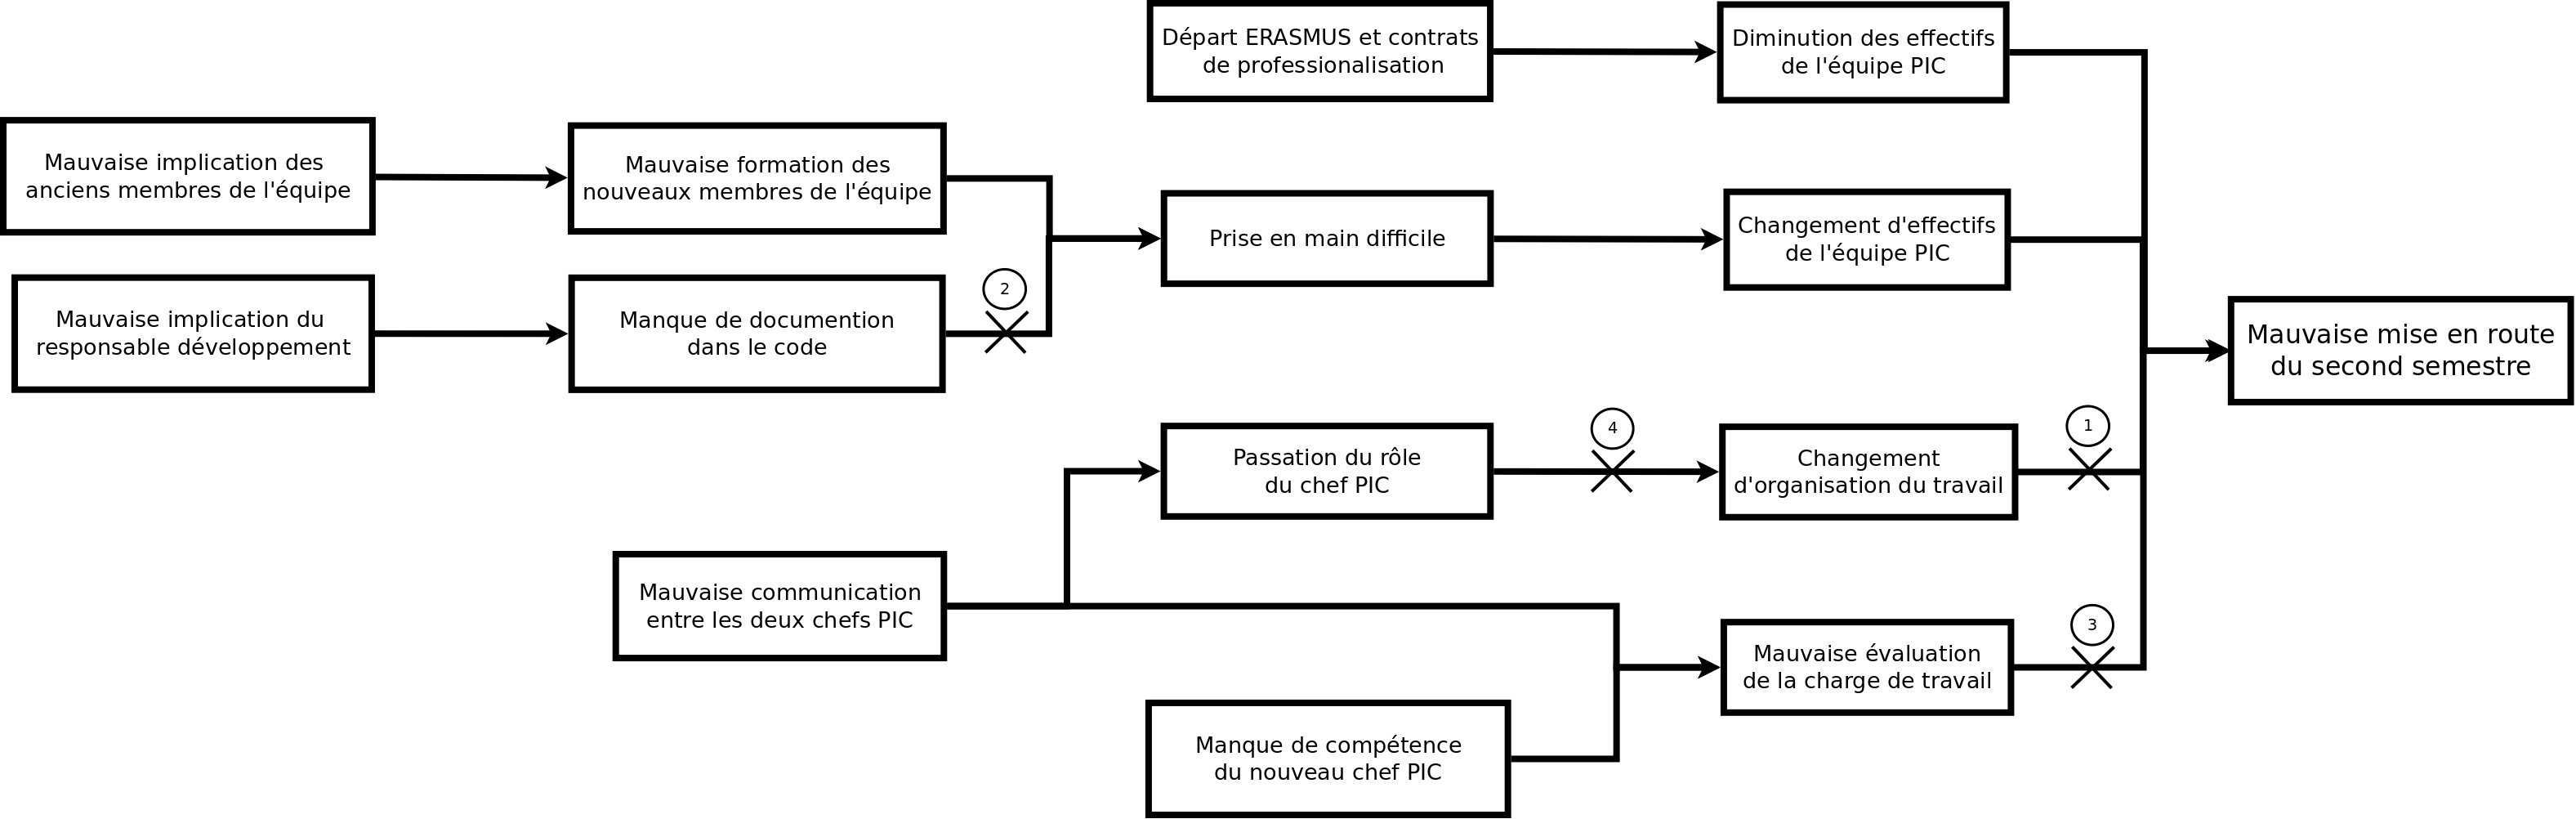
\includegraphics[scale=1.5]{images/AnalyseRisque_nPourquoi_FDR006}
	\caption{\label{risque Mauvaise mise en route du second semestre}risque de Mauvaise mise en route du second semestre - méthode des n pourquoi}
\end{figure}
\end{landscape}